\documentclass[12pt]{book} 
\usepackage[utf8]{inputenc} 
\usepackage[T1]{fontenc}
\usepackage[slovene]{babel} 	
\usepackage{amsmath} 
\usepackage{amssymb} 
\usepackage{amsthm}
\usepackage{bbm}
\usepackage{lmodern}
\usepackage{csquotes}
\usepackage{graphicx}
\usepackage{tikz}
\usepackage{pgfplots}
\usepackage{enumitem}
\usepackage{biblatex}           
\usepackage{hyperref}   
\usepackage{geometry}
\usepackage{float} 

\usepgfplotslibrary{fillbetween}
\pgfplotsset{compat=1.17}

\geometry{
    a4paper,
    left=30mm,
    right=30mm,
    top=30mm,
    bottom=40mm
}

\setlength{\parskip}{0.4em}
\linespread{1.2}

\makeatletter
\renewcommand{\maketitle}{
  \begin{titlepage}
    \begin{center}
      \vspace*{25mm} 
      \Huge\@title\par 
      \vspace{20mm} 
      \large\@author \\
      \vspace{140mm} 
      \large\@date\par 
    \end{center}
  \end{titlepage}
}
\makeatother

\usepackage{fancyhdr}
\makeatletter
\fancypagestyle{plain}{
  \fancyhf{}
  \renewcommand{\headrulewidth}{0pt} 
  \renewcommand{\footrulewidth}{0pt}
}
\makeatother

\pagestyle{fancy}
\fancyhf{}
\fancyhead[LE,RO]{\thepage}
\fancyhead[LO,RE]{\MakeUppercase{\leftmark}}
\fancyfoot{}
\renewcommand{\chaptermark}[1]{\markboth{#1}{}}
\renewcommand{\headrulewidth}{0.4pt} 

\def\n{\noindent}
\def\s{\vspace{10pt}}


\theoremstyle{definition}
\newtheorem{definicija}{Definicija}

\theoremstyle{plain}
\newtheorem{izrek}{Izrek}

\theoremstyle{plain}
\newtheorem{trditev}{Trditev}

\theoremstyle{plain}
\newtheorem{posledica}{Posledica}

\theoremstyle{remark}
\newtheorem*{opomba}{Opomba}

\usepackage{thmtools}
\declaretheoremstyle[
    spaceabove=10pt,
    spacebelow=10pt,
    bodyfont=\normalfont,
    headfont=\bfseries,
    postheadspace=0.5em,
    qed=$\lozenge$ 
]{example}
\declaretheorem[style=example, unnumbered]{zgled}


\usepackage{filemod}
\title{\Huge Verjetnost in statistika}
\author{\small Zapiski po predavanjih izr. prof. dr. Jaka Smrekarja \\ Napisal: \href{https://github.com/jonpascal/VIS-zapiski-predavanj}{Jon Pascal Miklavčič}}
\date{\filemodprintdate{\jobname}}

\makeatletter
\pgfmathdeclarefunction{erf}{1}{%
  \begingroup
    \pgfmathparse{#1 > 0 ? 1 : -1}%
    \edef\sign{\pgfmathresult}%
    \pgfmathparse{abs(#1)}%
    \edef\x{\pgfmathresult}%
    \pgfmathparse{1/(1+0.3275911*\x)}%
    \edef\t{\pgfmathresult}%
    \pgfmathparse{%
      1 - (((((1.061405429*\t -1.453152027)*\t) + 1.421413741)*\t 
      -0.284496736)*\t + 0.254829592)*\t*exp(-(\x*\x))}%
    \edef\y{\pgfmathresult}%
    \pgfmathparse{(\sign)*\y}%
    \pgfmath@smuggleone\pgfmathresult%
  \endgroup
}
\makeatother


\begin{document}

\frontmatter

\maketitle

\tableofcontents

\mainmatter

\part{Verjetnost}

\chapter{Slučajni vektorji}

\section{Slučajni vektorji}

\textbf{Spomnimo se:} 

\n \emph{Slučajna spremenljivka} na je taka funkcija $X: \Omega \to \mathbb{R}$, na verejetnostnem prostoru $(\Omega, \mathcal{F}, P)$, za katero so množice (praslike): 
$$
\{\omega \in \Omega: X(\omega) \leq x\}
$$
v $\mathcal{F}$, se pravi dogodki za vsak $x \in \mathbb{R}$

\n Oznaka:
$$
\{\omega \in \Omega: X(\omega) \leq x\} \equiv \{\omega \in \Omega \mid X(\omega) \in(-\infty, x]\} \equiv X^{-1}\left((-\infty, x]\right)
$$

\n Posledično je za slučajno spremenljivko $X$ definirana \emph{komulativna porazdelitvena funkcija} $F_X: \mathbb{R} \to [0,1]$:
$$
F_X(x)=P(X \leq x)=P\left(X^{-1}((-\infty, x])\right)
$$

\begin{definicija}
    \emph{Slučajni vektor} je taka preslikava $X=\left(X_1, \ldots, X_n\right): \Omega \to \mathbb{R}^n$ na verejetnostnem prostoru $(\Omega, \mathcal{F}, P)$, za katero so množice:
    $$
    \left\{X_1 \leq x_1, X_2 \leq x_2, \ldots, X_n \leq x_n\right\} :=\left\{\omega \in \Omega: X_1(\omega) \leq x_1, \ldots, X_n(\omega) \leq x_n\right\}
    $$
    v $\mathcal{F}$, se pravi dogodki za vse $n$-terice $x = \left(x_n, \ldots, x_n\right) \in \mathbb{R}^n$.
\end{definicija}

\n Oznaka: 
$$
\begin{aligned}
    \left\{X_1 \leq x_1, X_2 \leq x_2, \ldots, X_n \leq x_n\right\} &\equiv\left\{\omega \in \Omega: X_1(\omega) \leq x_1, \ldots, X_n(\omega) \leq x_n\right\} \\
    &\equiv \left\{X_1 \in\left(-\infty, x_1\right], \ldots, X_n \in\left(-\infty, x_n\right]\right\} \\ 
    &\equiv\{X \in\left(-\infty, x_1\right] \times \ldots \times\left(-\infty, x_n\right]\} \\
    &\equiv X^{-1}\left(\left(-\infty, x_n\right] \times \ldots \times\left(-\infty, x_n\right]\right)
\end{aligned}
$$

\begin{definicija}
    \emph{Komulativna porazdelitvena funkcija slučajnega vektorja} je funkcija $F_X: \mathbb{R}^n \to [0,1]$:
    $$
    F_X(x) \equiv F_{\left(X_1, \ldots, X_n\right)}\left(x_1, \ldots, x_n\right)=P\left(X_1 \leq x_1, \ldots, X_n \leq x_n\right)
    $$
\end{definicija}

\n \textbf{Lastnosti komulativne porazdelitvene funkcije:}

\begin{enumerate}
    \item ~ \vspace{-27.5pt}
    \begin{flalign*}
        \lim _{x_1 \to-\infty} F_{X}\left(x_1, \ldots, x_n\right)&=\lim _{x_1 \to-\infty} P\left( \vphantom{\vec X}X \in\left(-\infty, x_1\right] \times \right. \underbrace{\cdots \times\left(-\infty, x_n\right]}_{K}\left. \vphantom{\vec X} \right) & \\
        &=\lim _{n \to \infty} P\left(X \in(-\infty,-n] \times K\right) \tag{$\star$} & \\
        &=P\left(\bigcap_{n=1}^{\infty}\{X \in(-\infty,-n] \times K\}\right) & \\
        &=P\left(\vphantom{\bigcap_{n=1}^{\infty}} X \in \right. \underbrace{\bigcap_{n=1}^{\infty}(-\infty,-n] \times K}_{=\emptyset}\left. \vphantom{\bigcap_{n=1}^{\infty}} \right) & \\
        &=0&
    \end{flalign*}

    Kjer smo v $(\star)$  vrstici uporabili zveznost $P$ oziroma:
    $$
    \lim_{n \to \infty} P\left(E_n\right) = P\left(\bigcup_{n=1}^{\infty} E_n\right) \quad \text{za} \quad E_1 \supseteq E_2 \supseteq E_3 \supseteq \cdots
    $$
    Ta limita velja, tudi če proti $\infty$ pošljemo poljuben $x_i$. Velja še: 
    \begin{flalign*}
        \lim _{\left(x_1, \ldots, x_n\right) \to(\infty, \ldots, \infty)} F_{X}\left(x_1, \ldots, x_n\right)&=\lim _{n \to \infty} P(X\in(-\infty, n] \times \cdots \times(-\infty, n]) & \\
        &=P\left(\bigcup_{n=1}^{\infty} \{ X_1 \leq n, \ldots, X_n \leq n\} \right) & \\
        &=P\left( X \in \mathbb{R}^n \right) & \\
        &=P(\Omega) & \\
        &=1 &
    \end{flalign*}

    \newpage

    \item \emph{Monotnost:} če je $x_i \leq y_i$ za vse $i \in\{1, \ldots, n\}$, potem je: 
    $$
    F_{X}(x) \leq F_{X}(y)
    $$
    \begin{proof}
        Sledi iz monotonosti verjetnostne preslikave.  
    \end{proof}
    \item \emph{Zveznost z desne:} 
    $$
    \lim _{y \downarrow x} F_{X}(y)=F_{X}(x)
    $$
    Tukaj $y \downarrow x$ interpretiramo kot $y_i \downarrow x_i$ za vse $i \in\{1, \ldots, n\}$.
\end{enumerate}

\n Lastnosti 1., 2. in 3. karakterizirajo družino (abstraktnih) komulativnih porazdelitvenih funkcij v primeru slučajne spremenljivke t.j. $n=1$. V večrazsežnem primeru to ne drži. Poglejmo si $n=2$. Za $a<b$ in $c<d$ izračunajmo:
$$
P((X, Y) \in (a, b] \times (c, d]) = F_{(X, Y)}(b, d) - F_{(X, Y)}(a, d) -F_{(X, Y)}(b, c) + F_{(X, Y)}(a, c)
$$

\begin{figure}[H]
    \centering
    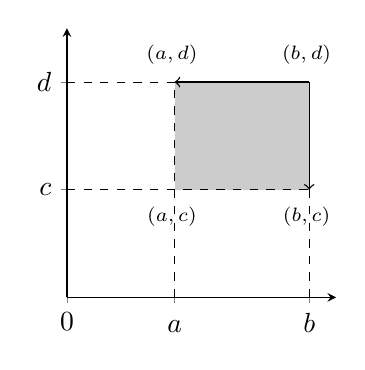
\begin{tikzpicture}

        \definecolor{siva}{rgb}{0.8, 0.8, 0.8}

        \begin{axis}[
            axis lines = left,
            domain=0:1,
            samples=500,
            height=5cm,
            width=5cm,
            xmin=0, xmax=1,
            ymin=0, ymax=1,
            xtick={0, 0.4, 0.9},
            ytick={0.4, 0.8},
            xticklabels={0, $\vphantom{b}a$, $b$},
            yticklabels={$c$, $d$}
        ]

        \fill[siva] (0.4, 0.4) rectangle (0.9, 0.8);

        \draw[dashed] (0.4, 0) -- (0.4, 0.8);
        \draw[dashed] (0.9, 0) -- (0.9, 0.8);
        \draw[dashed] (0, 0.4) -- (0.9, 0.4);
        \draw[dashed] (0, 0.8) -- (0.9, 0.8);
        \draw[->, line width=0.5pt] (0.9,0.8) -- (0.4,0.8);
        \draw[->, line width=0.5pt] (0.9,0.8) -- (0.9,0.4);

        \node at (0.89,0.9) {\scriptsize $(b, d)$};
        \node at (0.39,0.9) {\scriptsize $(a, d)$};
        \node at (0.89,0.3) {\scriptsize $(b, c)$};
        \node at (0.39,0.3) {\scriptsize $(a, c)$};
    
        \end{axis}
    \end{tikzpicture}

    \caption{$P((X, Y) \in(a, b] \times(c, d])$}
    \label{fig:1}
\end{figure}

\n Ker je to verjetnost mora veljati: 
\begin{align}
    F_{(X, Y)}(b, d) - F_{(X, Y)}(a, d) - F_{(X, Y)}(b, c) + F_{(X, Y)}(a, c) \geq 0 \tag{$4$} 
\end{align}

\begin{zgled}
    $$
    F(x, y)=
    \begin{cases}
        1 &; x \geq 1, y \geq 1 \\
        \frac{2}{3} &; x \geq 1, y \in[0,1) \\
        \frac{2}{3} &; x \in[0,1), y \geq 1 \\
        0 &; \text {sicer}
    \end{cases}
    $$

    \begin{figure}[H]
        \centering
        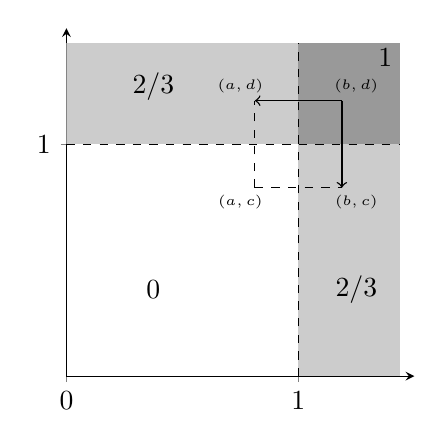
\begin{tikzpicture}
    
            \definecolor{siva1}{rgb}{0.8, 0.8, 0.8}
            \definecolor{siva2}{rgb}{0.6, 0.6, 0.6}
    
            \begin{axis}[
                axis lines = left,
                domain=0:2,
                samples=500,
                height=6cm,
                width=6cm,
                xmin=0, xmax=1.2,
                ymin=0, ymax=1.2,
                xtick={0, 0.8},
                ytick={0.8},
                xticklabels={0, 1},
                yticklabels={1}
            ]
    
            \fill[siva1] (0, 0.8) rectangle (0.8, 1.15);
            \fill[siva1] (0.8, 0.8) rectangle (1.15, 0);
            \fill[siva2] (0.8, 0.8) rectangle (1.15, 1.15);
    
            \draw[dashed] (0.8, 0) -- (0.8, 1.15);
            \draw[dashed] (0, 0.8) -- (1.15, 0.8);
            \draw[->, line width=0.5pt] (0.95,0.95) -- (0.65,0.95);
            \draw[->, line width=0.5pt] (0.95,0.95) -- (0.95,0.65);
            \draw[dashed] (0.65, 0.65) -- (0.65, 0.95);
            \draw[dashed] (0.65, 0.65) -- (0.95, 0.65);
            
            \node at (1,1) {\tiny $(b, d)$};
            \node at (0.6,1) {\tiny $(a, d)$};
            \node at (1,0.6) {\tiny $(b, c)$};
            \node at (0.6,0.6) {\tiny $(a, c)$};
            \node at (0.3,0.3) {$0$};
            \node at (0.3,1) {$2/3$};
            \node at (1,0.3) {$2/3$};
            \node at (1.1,1.1) {$1$};
        
            \end{axis}
        \end{tikzpicture}
    
        \caption[...]{Verjetnost $P((X, Y) \in (a, b] \times (c, d])$ za to k.p.f. \footnotemark}
        \label{fig:2}
    \end{figure}

    \footnotetext{k.p.f. je okrajšava za kumulativno porazdelitveno funkcijo. To se v skripti pojavi še večkrat.}

    \n Funkcija sicer zadošča lastnostim 1., 2. in 3., ampak za pravokotnik $(a, b] \times(c, d]$, kot na skici velja: 
    $$
    F(b, d)-F(a, d)-F(b, c)+F(a, c)=1-\frac{2}{3}-\frac{2}{3}+0<0
    $$
    Torej ne more biti komulativna porazdelitvena funkcija. 
\end{zgled}

\begin{izrek}
    Če $F: \mathbb{R}^2 \rightarrow[0,1]$ zadošča lastnostim $1., 2., 3.$ in $4.$ $(\text{velja } F(b, d)-F(a, d)-F(b, c)+F(a, c) \geq 0$, za vse četverice $a<b$ in $c<d)$, potem je $F$ komulativna porazdelitvena funkcija nekega slučajnega vektorja $(X,Y): \Omega \to \mathbb{R}^2$. 
\end{izrek}

\n Očitna posplošitev velja tudi za $n \geq 3$. 

\begin{trditev}
    Če je $X=\left(X_1, \ldots, X_n\right)$ slučajni vektor, so vsi podvektorji tudi slučajni vektorji.
\end{trditev}

\begin{proof}
    Na primer, za podvektor $\left(X_1, \ldots, X_{n-1}\right)$: 
    \begin{align}
        \left\{X_1 \leq x_1, \ldots, X_{n-1} \leq x_{n-1}\right\}=\bigcup_{k=1}^{\infty}\left\{X_1 \leq x_1, \ldots, X_{n-1} \leq x_{n-1}, X_n \leq k\right\} \tag{$\star$} 
    \end{align}
\end{proof}

\n Posebej sledi, da so komponente slučajnih vektorjev, funkcije $X_1, X_2, \ldots, X_n$, slučajne spremenljivke. Iz $(\star)$ je očitno tudi, da komulativne porazdelitvene funkcije podvektorjev dobimo tako, da ustrezne kooridante pošljemo proti $\infty$:
$$
F_{\left(X_1, \ldots, X_{n-1}\right)}\left(x_1, \ldots, x_{n-1}\right)=\lim _{x_n \to \infty} F_{\left(X_1, \ldots, X_n\right)}\left(x_1, \ldots, x_n\right)
$$
Komulativne porazdelitvene funkcije $F_{X_i}$ imenujemo tudi \emph{robne} ali \emph{marginale} komulativne porazdelitvene funckije (glede na $F_{(X_1, \ldots, X_n)}$). 

\begin{opomba}
    Naj bo $X: \Omega \to \mathbb{R}$ s.s.\footnote[2]{s.s. je okrajšava za slučajno spremenljivko. To se v skripti pojavi še večkrat.} Potem so naslednje množice dogodki:
    \begin{itemize}
        \item ~ \vspace{-27pt}
        \begin{flalign*}
            \{X \in(a, b]\} &=\{X \in(-\infty, b]\} \setminus \{X \in(-\infty, a]\} & \\ 
            &=\{X \in(-\infty, b]\} \cap\{X \in(-\infty, a]\}^c &
        \end{flalign*}
        \item $\{X \in(a, b)\}$, saj je to enako $\bigcup_{n=1}^{\infty}\left\{X \in\left(a, c_n\right]\right\}$ za $c_n \uparrow b$
        \item $\{X \in[a, b]\}=\bigcap_{n=1}^{\infty}\left\{X \in\left(a-\frac{1}{n}, b+\frac{1}{n}\right)\right\}$
        \item $\{X=x\} = \{X \in (x-1, x] \} \setminus \{ X \in (x-1, x)\}$
    \end{itemize}
    Zgornje lahko “kombiniramo” (števne unije, komplementi, preseki). Izkaže se, da obstajajo verjetnosti $P(X \in \mathcal{B})$, kjer je $\mathcal{B} \subseteq \mathbb{R}$ poljubna Borelova množica. 
\end{opomba}

\begin{opomba}
    Pripomnimo, da podobno velja za slučajni vektor $X$. Množice: 
    $$
    \{X \in \mathcal{B}\}=X^{-1}(\mathcal{B}) \subseteq \Omega
    $$
    so dogodki za Borelove množice $\mathcal{B} \subseteq \mathbb{R}^n$
\end{opomba}

\begin{zgled}[Borelove množice]
    ~

    \begin{enumerate}
        \item $\subseteq \mathbb{R}$
        \begin{itemize}
            \item $(a, b), (-\infty, b), \ldots$ vsi intervali;
            \item $\{x\}=(x-1,x]\setminus(x-1,x)$ singeltoni;
            \item Števne unije Borelovih množic;
            \item Števni preseki Borelovih množic;
            \item Komplementi Borelovih množic.
        \end{itemize}
        \item $\subseteq \mathbb{R}^2$
        \begin{itemize}
            \item Krogle;
            \item Pravokotniki;
            \item Enoelementne množice;
            \item Unije, preseki, komplemeti kot v $\mathbb{R}$;
            \item Če je $G: \mathbb{R}^2 \rightarrow \mathbb{R}^2$ zvezno parcialno odvedljiva bijekcija, je $G(\mathcal{B})$ Borelova za vsako Borelovo množico $\mathcal{B}$.
        \end{itemize}
    \end{enumerate}
\end{zgled}

\section{Zvezni slučajni vektorji}

\begin{definicija}
    Slučajni vektor $X: \Omega \to \mathbb{R}^n$ ima zvezno gostoto, če obstaja taka “zvezna” funkcija $f_{X}: \mathbb{R}^n \rightarrow[0, \infty)$, da zanjo velja: 
    $$
    P(X \in \mathcal{B})=\int_{\mathcal{B}} f_{X}\left(x_1, \ldots, x_n\right) \, d x_1 \cdots d x_n = \int_{\mathcal{B}}f_X(x) \, dx
    $$
    za vsako Borelovo množico $\mathcal{B} \subseteq \mathbb{R}^n$.
\end{definicija}

\n Mislimo si, da gre za posplošeni Reimannov integral. Zvezna funkcija $f_X: \mathbb{R}^n \to [0,\infty)$  je taka, pri kateri je množica točk nezveznosti zanemarljiva za $n$-terni integral. Če ima slučajni vektor $X$ “zvezno” gostoto, pravimo, da je zvezen. V tem primeru je $F_X: \mathbb{R}^n \to [0,1]$ \emph{zvezna} funkcija.

\begin{zgled}
    $X \sim \operatorname{U}(a, b)$ (enakomerna zvezna porazdelitev na $(a,b)$). Vse točke so “enako verjetne”. Natančneje za $a \leq c<d \leq b$: 
    $$
    \begin{aligned}
        P\left(X \in(c, d) \right)=\int_c^d f_{\operatorname{U}(a, b)}(x) \, d x, \quad \text{kjer je} \quad f_{\operatorname{U}(a, b)}(x)&=\frac{1}{b-a} \cdot \mathbbm{1}_{(a, b)}(x) \\
        &= \begin{cases}\frac{1}{b-a} &; x \in (a,b) \\ 0 &; x \notin (a,b)\end{cases}
    \end{aligned}
    $$

    \begin{figure}[H]
        \centering
        \begin{tikzpicture}
            \begin{axis}[
                axis lines = left,
                domain=-3:3,
                samples=500,
                height=4cm,
                width=10cm,
                xmin=-3, xmax=3,
                ymin=0, ymax=0.5,
                ytick={0.3},
                xtick={-2, 2},
                yticklabels={$\frac{1}{b-a}$},
                xticklabels={$a$, $b$},
                yticklabel style={xshift=0cm}
            ]
            
            \draw[line width=1pt] (-3, 0) -- (-2, 0);
            \draw[->, line width=1pt] (-2, 0.3) -- (2, 0.3);
            \draw[->, line width=1pt] (2, 0.3) -- (-2, 0.3);
            \draw[line width=0.5pt] (-3, 0) -- (3, 0);
            
            \draw[dashed] (-2, 0) -- (-2, 0.3);
            \draw[dashed] (2, 0) -- (2, 0.3);
            \draw[dashed] (-3, 0.3) -- (2, 0.3);
            
            \end{axis}
        \end{tikzpicture}

        \caption{$f_X(x)$ za enakomerno porazdelitev}
        \label{fig:3}
    \end{figure}
\end{zgled}

\begin{definicija}
    Za abstraktno množico $M$ in $A \subseteq M$ je $\mathbbm{1}_A: M \to \{ 0, 1\}$ \emph{indikator množice} $A$ funkcija: 
    $$
    \mathbbm{1}_A(m)= \begin{cases}1 &; m \in A \\ 0 &; m \notin A\end{cases}
    $$
\end{definicija}

\begin{opomba}
    Velja: $P(X \in A)=E\left(\mathbbm{1}_A(X)\right)$
\end{opomba}

\begin{zgled}
    V primeru $X \sim \operatorname{U}(a,b)$ je gostota $X$ tudi: 
    $$
    f_X(x)=\begin{cases}
        \frac{1}{b-a} &; x \in(a, b) \setminus\left\{\frac{a+b}{2}\right\} \\
        \, 42 &; x=\frac{a+b}{2} \\
        \, \, \, 0 &; x \notin(a, b)
        \end{cases}
    $$
    \begin{figure}[H]
        \centering
        \begin{tikzpicture}
            \begin{axis}[
                axis lines = left,
                domain=-3:3,
                samples=500,
                height=4cm,
                width=10cm,
                xmin=-3, xmax=3,
                ymin=0, ymax=0.55,
                ytick={0.2, 0.5},
                xtick={-2, 0, 2},
                yticklabels={$\frac{1}{b-a}$, 42},
                xticklabels={\vphantom{$\frac{a+b}{2}$}$a$, $\frac{a+b}{2}$, \vphantom{$\frac{a+b}{2}$}$b$},
                yticklabel style={xshift=0cm}
            ]
            
            \draw[line width=1pt] (-3, 0) -- (-2, 0);
            \draw[->, line width=1pt] (-2, 0.2) -- (0, 0.2);
            \draw[->, line width=1pt] (0, 0.2) -- (-2, 0.2);
            \draw[->, line width=1pt] (0, 0.2) -- (2, 0.2);
            \draw[->, line width=1pt] (2, 0.2) -- (0, 0.2);
            \draw[line width=1pt] (2, 0) -- (3, 0);
            \draw[line width=0.5pt] (-3, 0) -- (3, 0);
            
            \draw[dashed] (-2, 0) -- (-2, 0.2);
            \draw[dashed] (2, 0) -- (2, 0.2);
            \draw[dashed] (-3, 0.2) -- (2, 0.2);
            \draw[dashed] (0, 0) -- (0, 0.47);
            \draw[dashed] (-0.08 , 0.5) -- (-5, 0.5);

            \addplot[mark=*, mark size=1pt] coordinates {(0,0.5)};
            
            \end{axis}
        \end{tikzpicture}

        \caption{$f_X(x)$ za enakomerno porazdelitev}
        \label{fig:4}
    \end{figure}
\end{zgled}

\begin{zgled}
    $D = \left\{(x, y) \in \mathbb{R}^2 \mid x^2+y^2<1\right\}$ odprt enotski krog. Pravimo, da $(X, Y) \sim \operatorname{U}(D)$, če ima gostoto: 
    $$
    f_{(X, Y)}(x, y)=\frac{1}{\pi} \cdot \mathbbm{1}_D(x, y)
    $$
    Množica točk nezveznosti zgornje gostote je enotska krožnica. To je zanemarljiva množica za $\int_{\mathbb{R}^2}$.
\end{zgled}

\n \textbf{Oglejmo si dvorazsežen primer ($n=2$):}

\n Za $(X, Y): \Omega \to \mathbb{R}^2$ z gostoto $f_{(X, Y)}: \mathbb{R}^2 \to [0, \infty)$ velja: 
\begin{align*}
    F_{(X, Y)}(x, y)&=P((X, Y) \in(-\infty, x] \times(-\infty, y]) \\
    &=\int_{(-\infty, x] \times(-\infty, y]} f_{(X, Y)}(u, v) \, d u d v \\
    &=\int_{-\infty}^x \int_{-\infty}^y f_{(X, Y)}(u, v) \, d v d u \tag{$\star$} \\
    &=\int_{-\infty}^y \int_{-\infty}^x f_{(X, Y)}(u, v) \, d u d v
\end{align*}
Kjer smo v $(\star)$ vrstici uporabili Fubinijev izrek (integral mora biti absolutno konvergenten).

\n Robni komulativni porazdelitveni funkciji se glasita: 
$$
\begin{aligned}
    F_X(x)&=\lim _{y \rightarrow \infty} F_{(X, Y)}(x, y) \\
    &=\lim _{y \rightarrow \infty} \int_{-\infty}^y \int_{-\infty}^x f_{(X, Y)}(u, v) \, d u d v \\
    &=\int_{-\infty}^{\infty} \int_{-\infty}^x f_{(X, Y)}(u, v) \,d u d v \\
    &=\int_{-\infty}^x \int_{-\infty}^{\infty} f_{(X, Y)}(u, v) \, d v d u
\end{aligned}
$$
$$
\begin{aligned}
    F_Y(y)&=\lim _{x \rightarrow \infty} F_{(X, Y)}(x, y) \\
    &=\lim _{x \rightarrow \infty} \int_{-\infty}^x \int_{-\infty}^y f_{(X, Y)}(u, v) \, d u d v \\
    &=\int_{-\infty}^{\infty} \int_{-\infty}^y f_{(X, Y)}(u, v) \,d u d v \\
    &=\int_{-\infty}^y \int_{-\infty}^{\infty} f_{(X, Y)}(u, v) \, d v d u
\end{aligned}
$$
Od tod sledita robni gostoti: 
$$
f_X(x)=F_X^{\prime}(x)=\int_{-\infty}^{\infty} f_{(X, Y)}(x, v) \, d v
$$
$$
f_Y(y)=F_Y^{\prime}(y)=\int_{-\infty}^{\infty} f_{(X, Y)}(u, y) \, d u
$$
V točkah odevljivosti k.p.f. $F$, oz. za skoraj vse $x$ oz. $y$. 

\section{Dvofazna normalna porazdelitev}

Naj bo $\mu=\begin{bmatrix}\mu_1 \\ \mu_2 \end{bmatrix} \in \mathbb{R}^2$ in naj bo $\Sigma=\begin{bmatrix} \sigma_1^2 & \sigma_{12} \\ \sigma_{12} & \sigma_2^2\end{bmatrix}$, kjer je $\sigma_1, \sigma_2 \in(0, \infty)$ in $\sigma_{12} \in \mathbb{R}$, simetična pozitivno definitna $2 \times 2$ matirka ($\iff \det (\Sigma) > 0$). Tedaj ima slučajni vektor $(X,Y)$ dvorazsežno normalno porazdelitev s parametroma $\mu$ in $\Sigma$, če ima gostoto: 
$$
f_{(X,Y)}(x, y)=\frac{1}{2 \pi} \frac{1}{\sqrt{\operatorname{det} \Sigma}} \cdot \exp \left(-\frac{1}{2}\left\langle\Sigma^{-1}\left(\begin{bmatrix} x \\ y \end{bmatrix}-\begin{bmatrix} \mu_1 \\ \mu_2 \end{bmatrix}\right),\begin{bmatrix} x \\ y \end{bmatrix}-\begin{bmatrix} \mu_1 \\ \mu_2 \end{bmatrix} \right\rangle \right)
$$
Gostota $f_{X,Y}$ je zvezna povsod na $\mathbb{R}^2$. 

\begin{opomba}
    Pišemo $(X, Y) \sim \operatorname{N}(\mu, \Sigma)=N\left(\begin{bmatrix} \mu_1 \\ \mu_2 \end{bmatrix},\begin{bmatrix} \sigma_1^2 & \sigma_{12} \\ \sigma_{12} & \sigma_2^2 \end{bmatrix}\right)$.
\end{opomba}

\n Seveda je: 
$$
\Sigma^{-1}=\frac{1}{\sigma_1{ }^2 \sigma_2{ }^2-\sigma_{12}^2}\begin{bmatrix} \sigma_2^2 & -\sigma_{12} \\ -\sigma_{1 2} & \sigma_1^2 \end{bmatrix}
$$
Tako dobimo:  $\left\langle\Sigma^{-1}\left(\begin{bmatrix} x \\ y \end{bmatrix}-\begin{bmatrix} \mu_1 \\ \mu_2 \end{bmatrix}\right),\begin{bmatrix} x \\ y \end{bmatrix}-\begin{bmatrix} \mu_1 \\ \mu_2 \end{bmatrix}\right\rangle = (\star)$ prepišemo v: 

\begin{align*}
    \left\langle\Sigma^{-1}\begin{bmatrix} x - \mu_1 \\ y - \mu_2 \end{bmatrix},\begin{bmatrix} x - \mu_1 \\ y - \mu_2 \end{bmatrix}\right\rangle &= \frac{1}{\sigma_1^2 \sigma_2^2-\sigma_{12}^2} \left\langle \begin{bmatrix}\sigma_2^2 & -\sigma_{12} \\ -\sigma_{12} & \sigma_1^2 \end{bmatrix}\begin{bmatrix} x-\mu_1 \\ y-\mu_2 \end{bmatrix}, \begin{bmatrix} x-\mu_1 \\ y-\mu_2 \end{bmatrix}\right\rangle \\
    &= \frac{1}{\sigma_1^2 \sigma_2^2-\sigma_{12}^2} \left\langle \begin{bmatrix} \sigma_2^2\left(x-\mu_1\right)-\sigma_{12}\left(y-\mu_2\right) \\ \sigma_1^2\left(y-\mu_2\right)-\sigma_{12}\left(x \mu_1\right) \end{bmatrix}, \begin{bmatrix} x-\mu_1 \\ y-\mu_2 \end{bmatrix} \right\rangle \\
    &= \frac{\sigma_2^2\left(x-\mu_1\right)^2-2 \sigma_{12}\left(x-\mu_1\right)\left(y-\mu_2\right)+\sigma_1^2\left(y-\mu_2\right)^2}{\sigma_1^2 \sigma_2^2-\sigma_{12}^2}
\end{align*}

\n Vpeljemo $\rho=\frac{\sigma_{12}}{\sigma_1 \sigma_2}$. Ker je $\det \Sigma=\sigma_1{ }^2 \sigma_2{ }^2\left(1-\rho^2\right)$ je $\det \Sigma >0 \iff \rho^2<1$, oz. $\rho \in(-1,1)$. S parametrom $\rho$ lahko nadomestimo $\sigma_{12}$. Dobimo: 
$$
\scalebox{1}{$\left\langle\Sigma^{-1}\begin{bmatrix} x - \mu_1 \\ y - \mu_2 \end{bmatrix},\begin{bmatrix} x - \mu_1 \\ y - \mu_2 \end{bmatrix}\right\rangle = \frac{1}{1-\rho^2}\left(\left(\frac{x-\mu_1}{\sigma_1}\right)^2-2 \rho\left(\frac{x-\mu_1}{\sigma_1}\right)\left(\frac{y-\mu_2}{\sigma_2}\right)+\left(\frac{y-\mu_2}{\sigma_2}\right)^2\right)$}
$$
Ekvivalentno lahko torej normalno porazdelitev parametriziramo s parametri:
$$
\mu_1 \in \mathbb{R}, \mu_2 \in \mathbb{R}, \sigma_1 \in(0, \infty), \sigma_2 \in(0, \infty), \rho \in(-1,1)
$$
Dobimo: 
$$
\scalebox{1}{$f_{(X, Y)}(x, y)=\frac{1}{2 \pi \sigma_1 \sigma_2 \sqrt{1-\rho^2}} \exp\left(-\frac{1}{2\left(1-\rho^2\right)}\left(\left(\frac{x-\mu_1}{\sigma_1}\right)^2-2 \rho\left(\frac{x-\mu_1}{\sigma_1}\right)\left(\frac{y-\mu_2}{\sigma_2}\right)+\left(\frac{y-\mu_2}{\sigma_2}\right)^2\right)\right)$}
$$

\n Vidimo, da so nivojnice funkcije $f_{(X,Y)}$ krivulje, ki so elipse s središčem v $(\mu_1, \mu_2)$.

\n Oglejmo si poseben primer $\mu_1=\mu_2=0, \sigma_1=\sigma_2=1$ (ekvivalentno, obravnavamo gostoto transformacije $U=\frac{X-\mu_1}{\sigma_1}, V=\frac{Y-\mu_2}{\sigma_2}$). Nivojnice se krivulje: 
$$
\begin{aligned}
    u^2-2 \rho u v+v^2&=C\left(1-\rho^2\right) \\ 
    \left\langle\begin{bmatrix} 1 & -\rho \\ -\rho & 1 \end{bmatrix} \begin{bmatrix} u \\ v \end{bmatrix},\begin{bmatrix} u \\ v \end{bmatrix}\right\rangle&=C\left(1-\rho^2\right)
\end{aligned}
$$

\newpage

\n To je kvadratna forma oblike $q_A(x) = \langle Ax, x \rangle$. Izračunajmo lastni vrednosti matrike $A=\begin{bmatrix} 1 & -\rho \\ -\rho & 1 \end{bmatrix}$: 
$$
\begin{aligned}
    \det (A -\lambda I) &= \begin{vmatrix} 1 -\lambda & -\rho \\ -\rho & 1 -\lambda \end{vmatrix} \\
    &= (1 -\lambda)^2 - \rho^2 \\
    &=(1-\lambda - \rho)(1-\lambda + \rho)
\end{aligned}
$$
Lastni vrednosti sta $1 \pm \rho$.

\begin{flalign*}
    & \lambda_1=1-\rho:\begin{bmatrix} \rho & -\rho \\ -\rho & \rho \end{bmatrix}\begin{bmatrix} 1 \\ 1 \end{bmatrix} = \begin{bmatrix} 0 \\ 0 \end{bmatrix} \quad \implies \text{lastni vektor je} \quad \begin{bmatrix} 1 \\ 1 \end{bmatrix} \\ 
    &\lambda_1=1+\rho:\begin{bmatrix} -\rho & -\rho \\ -\rho & -\rho \end{bmatrix}\begin{bmatrix} -1 \\ 1 \end{bmatrix} = \begin{bmatrix} 0 \\ 0\end{bmatrix} \quad \implies \text{lastni vektor je} \quad \begin{bmatrix} -1 \\ 1 \end{bmatrix} 
\end{flalign*}

\begin{figure}[H]
    \centering
    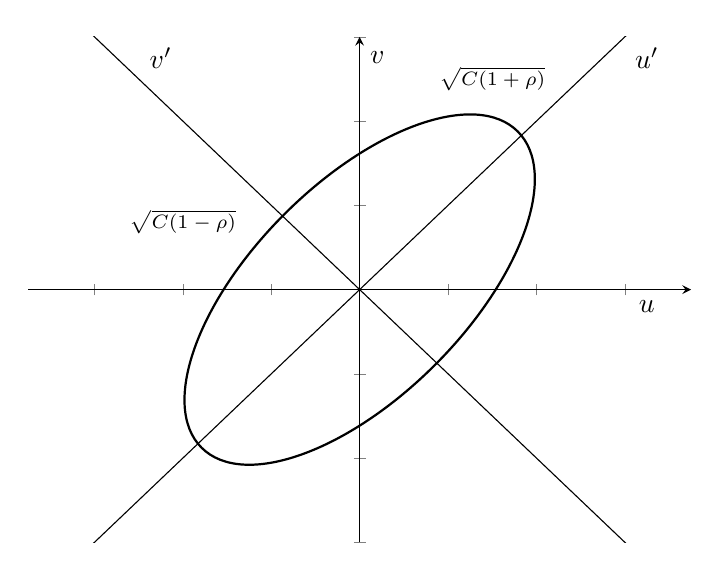
\begin{tikzpicture}
        \begin{axis}[
            axis lines = middle,
            domain=-3:3,
            samples=500,
            height=8cm,
            width=10cm,
            xmin=-3.75, xmax=3.75,
            ymin=-3, ymax=3,
            xtick={},
            ytick={},
            xticklabels={},
            yticklabels={}
        ]
        
        \def\C{4} 
        \def\angle{45}
        \def\lambdamajor{sqrt(\C*(1+0.6))}
        \def\lambdaminor{sqrt(\C*(1-0.6))}

        \draw[thick] (0,0) ellipse [x radius=\lambdamajor, y radius=\lambdaminor, rotate=\angle];

        \draw[->] (-5,-5) -- (5,5) node[right] {$u'$};
        \draw[->] (5,-5) -- (-5,5) node[left] {$v'$};

        \node at (-2,0.8) {\scriptsize $\sqrt{C(1-\rho)}$};
        \node at (1.5,2.5) {\scriptsize $\sqrt{C(1+\rho)}$};

        \node at (3.25, -0.2) {$u$};
        \node at (0.2, 2.75) {$v$};
        \node at (3.25, 2.75) {$u^{\prime}$};
        \node at (-2.25, 2.75) {$v^{\prime}$};

        \end{axis}
    \end{tikzpicture}

    \caption{Nivojnica $\operatorname{N}\left(\begin{bmatrix} 0 \\ 0 \end{bmatrix}, \begin{bmatrix} 1 & \rho \\ \rho & 1 \end{bmatrix}\right)$}
    \label{fig:5}
\end{figure}

\n V koordinatah $\begin{bmatrix}
    u^{\prime} \\
    v^{\prime}
    \end{bmatrix}=\begin{bmatrix}
    \frac{1}{\sqrt{2}} & \frac{1}{\sqrt{2}} \\
    -\frac{1}{2} & \frac{1}{\sqrt{2}}
    \end{bmatrix}\begin{bmatrix}
    u \\
    v
    \end{bmatrix}$ dobimo enačbo:
$$
(1-\rho) u^{\prime 2}+(1+\rho) v^{\prime 2}=C\left(1-\rho^2\right) \iff \frac{u^{\prime 2}}{C(1+\rho)}+\frac{v^{\prime 2}}{C(1-\rho)}=1
$$

%\begin{figure}[H]
%    \centering
%    \begin{tikzpicture}
%        \begin{axis}[
%            view={40}{40},
%            grid=major,
%            domain=-3:3, 
%            y domain=-3:3,
%            zmax=0.23,
%            samples=50,
%            height=10cm,
%            width=10cm,
%            colormap/cool,
%            xlabel={$x$}, ylabel={$y$}, zlabel={$z$},
%            xtick=\empty, ytick=\empty, ztick=\empty,
%            axis lines=center
%        ]
%        
%        \pgfmathsetmacro\rho{0.6}  
%        \pgfmathsetmacro\a{sqrt(1-\rho^2)}  
%        
%        \addplot3[
%            surf,
%            opacity=0.7,
%        ]
%        {exp(-0.5*(x^2 + y^2 - 2*\rho*x*y) / \a^2) / (2*pi*\a)};
%
%        \addplot3 [
%            thick, orange, dashed,
%            samples=50,
%            samples y=0,
%            domain=0:2*pi,
%        ]
%        ({sqrt((-2 * (\a)^2 * ln(0.1 * pi * \a)) / (1 - \rho * sin(2 * deg(x)))) * cos(deg(x))},
%        {sqrt((-2 * (\a)^2 * ln(0.1 * pi * \a)) / (1 - \rho * sin(2 * deg(x)))) * sin(deg(x))}, 
%        {0.05}); 
%
%        \end{axis}
%    \end{tikzpicture}
%
%    \caption{Gostota $\operatorname{N}\left(\begin{bmatrix} 0 \\ 0 \end{bmatrix}, \begin{bmatrix} 1 & \rho \\ \rho & 1 \end{bmatrix}\right)$ z nivojnico}
%    \label{fig:6}
%\end{figure}

\n Naj bo $(X,Y) \sim N\left(\begin{bmatrix} \mu_1 \\ \mu_2 \end{bmatrix},\begin{bmatrix} \sigma_1^2 & \sigma_{12} \\ \sigma_{12} & \sigma_2^2 \end{bmatrix}\right)$. Izkaže se, da za robni porazdelitvi velja: 
$$
X \sim N\left(\mu_1, \sigma_1{ }^2\right) \quad \text {in} \quad Y \sim N\left(\mu_2, \sigma_2^2\right)
$$
Nadalje se izkaže, da je $\sigma_{1 2}=K(X, Y)$. Posledično je $\rho$ t.i. Pearsonov korelacijski koeficient. 

\begin{opomba}
    Pripomnimo, da sledi, da porazdelitev vektorja $(X,Y)$ ni določena z robnima porazdelitvama. 
\end{opomba}

\begin{zgled}
    Oglejmo si primer $(X,Y) \sim N\left(\begin{bmatrix} 0 \\ 0 \end{bmatrix},\begin{bmatrix} 1 & \rho \\ \rho & 1 \end{bmatrix}\right)$. Tedaj se gostota $(X, Y)$ glasi:
    $$
    f_{(X, Y)}(x, y)=\frac{1}{2 \pi} \cdot e^{-\frac{1}{2\left(1-\rho^2\right)}\left(x^2-2 \rho x y+y^2\right)}
    $$
    $\rho = 0 \implies$ standardna dvorazsežna normalna porazdelitev.
\end{zgled}

\n \textbf{Posplošitev:}

\n Pravimo, da ima vektor $X=\left(X_1, \ldots, X_n\right)$ $n$-razsežno normalno porazdelitev s parametroma $\mu \in \mathbb{R}^n$ in $\Sigma \in \mathbb{R}^{n \times n}$ (simetrična in poz. definitna), če ima gostoto: 
$$
f_{X}(x)=(2 \pi)^{-\frac{n}{2}}(\det \Sigma)^{-\frac{1}{2}} \exp\left(-\frac{1}{2}\left\langle\Sigma^{-1}(x-\mu), x-\mu\right\rangle\right)
$$

\chapter{Neodvisnost}

\begin{definicija}
    Slučajne spremenljivke $X_1, \ldots, X_n$, so neodvisne, če velja: 
    \begin{align*}
        F_{X}\left(x_1, \ldots, x_n\right)=F_{X_1}\left(x_1\right) \cdot F_{X_2}\left(x_2\right) \cdots F_{X_n}\left(x_n\right) \tag{$\star$} 
    \end{align*}
    za vse realne $n$-terice $\left(x_1, \ldots, x_n\right) \in \mathbb{R}^n$.
\end{definicija}

\n Enakost $(\star)$ lahko prepišemo v: 
$$
P\left(X \in\left(-\infty, x_1\right] \times \ldots \times\left(-\infty, x_n\right]\right)=P\left(X_1 \in\left(-\infty, x_1\right]\right) \cdots  P\left(X_n \in\left(-\infty, x_n\right]\right)
$$

\n Izkaže se, da so komponente vektorja $X$ neodvisne natanko tedaj, ko velja:
$$
P\left(X_1 \in B_1, X_2 \in B_2, \ldots, X_n \in B_n\right)=P\left(X_1 \in B_1\right) \cdot P\left(X_2 \in B_2\right) \cdots P\left(X_n \in B_n\right)
$$
za vse $n$-terice Borelovih množic $B_i \subseteq \mathbb{R}$.

\n Torej za slučajni spremenljivki $X, Y$ velja, da sta neodvisni natanko tedaj, ko: 
$$
P(X \in A, Y \in B)=P(X \in A) \cdot P(Y \in B)
$$
za vse intervale $A,B \subseteq \mathbb{R}$

\n Spomnimo se, da so dogodki $E_1, E_2, \ldots , E_n$ neodvisni:
$$
P\left(E_{i_1} \cap \cdots \cap E_{i_k}\right)=P\left(E_{i_1}\right) \cdots P\left(E_{i_k}\right)
$$
za $\forall k \in \{2, 3, \ldots, n\}$ in vsako $k$-terico $i_1<i_2<\ldots<i_k$.

\begin{opomba}
    Če so $X_1, \ldots, X_n$ neodvisne, so tudi paroma neodvisne, t.j. neodvisni sta $X_i$ in $X_j$ za vsak par $i \neq j$. Obratno ne velja v splošnem. 
\end{opomba}

\begin{trditev}
    Naj ima slučajni vektor $(X,Y)$ “zvezno” gostoto $f_{(X,Y)}:\mathbb{R}^2 \to [0, \infty)$. $X$ in $Y$ sta neodvisni $\iff$
    $$
    f_{(X, Y)}(x, y)=f_X(x) \cdot f_Y(y)
    $$
    za skoraj vse realne pare $(x,y) \in \mathbb{R}^2$.
\end{trditev}

\begin{proof}
    Definicija neodvisnosti pravi: 
    $$
    P((X, Y) \in(-\infty, x] \times(-\infty, y])=P(X \in(-\infty, x]) P(Y \in(-\infty, y])
    $$
    Oziroma: 
    $$
    \begin{aligned}
      \int_{(-\infty, x] \times(-\infty, y]} f_{(X, Y)}(u, v) \, d u d v&=\int_{(-\infty, x]} f_X(u) \, d u \int_{(-\infty, y]} f_Y(v) \, d v  \\
      \int_{-\infty}^x \int_{-\infty}^y f_{(X, Y)}(u, v) \, d v d u&=\int_{-\infty}^x f_X(u) \, d u \int_{-\infty}^y f_Y(v) \, d v
    \end{aligned}
    $$
    $(\implies)$ Uporabimo osnovni izrek analize in odvajamo najprej po $x$:
    $$
    \int_{-\infty}^y f_{(X, Y)}(x, y) \, d v=f_X(x) \int_{-\infty}^y f_Y(v) \, d v
    $$
    Odvajati smemo skoraj v vseh točka $x \in \mathbb{R}$, saj gostote niso vedno povsod zvezne. Odvjamo še po $y$: 
    $$
    f_{(X, Y)}(x, y)=f_X(x) f_Y(y)
    $$
    Velja za skoraj vse $x$ in $y$.\footnote[3]{Enakost za skoraj vse $x$ in $y$ pomeni enakost za vse integrale po Borelovih množicah.}

    \n $(\impliedby)$ Če veja $f_{(X, Y)}(u, v)=f_X(u) f_Y(v)$ za skoraj vse $u,v$ veja tudi: 
    $$
    \int_{(-\infty, x] \times(-\infty, y]} f_{(X, Y)}(u, v) \, d u d v=\int_{(-\infty, x] \times(-\infty, y]} f_X(u) \cdot f_Y(v) \, d u d v
    $$
    za vse\footnote[4]{Če sta funkciji skoraj povsod enaki je integral funkcij enak povsod.} $x$ in $y$. Leva starn je $F_{(X,Y)}(x,y)$, na desni strani pa dvojni integral spremeninmo v dvakratnega: 
    $$
    \begin{aligned}
        \int_{(-\infty, x] \times(-\infty, y]} f_X(u) \cdot f_Y(v) \, d u d v &= \int_{(-\infty, x]} f_X(u) \int_{(-\infty, y]} f_Y(v) \, d v d u\\
        &=\int_{(-\infty, x]} f_X(u) \, d u \int_{(-\infty, y]} f_Y(v) \, d v \\
        &= F_X(x) \cdot F_Y(y)
    \end{aligned}
    $$
\end{proof}

\begin{posledica}
    Če je $(X,Y) \sim N\left(\begin{bmatrix}\mu_1 \\ \mu_2 \end{bmatrix}, \begin{bmatrix} \sigma_1^2 & \sigma_{12} \\ \sigma_{12} & \sigma_2^2 \end{bmatrix}\right)$ potem sta $X$ in $Y$ neodvisni $\iff$ $\sigma_{12} \iff \rho = 0$.
\end{posledica}

\begin{proof}
    $(\implies)$ Spomnimo se, da ima $(X,Y)$ gostoto:
    $$
    f_{(X,Y)}(x,y) = \frac{1}{2 \pi} \cdot \frac{1}{\sqrt{\det \Sigma}} \cdot e^{-\frac{1}{2}\left\langle\Sigma^{-1}\left(\vec{x} - \vec{\mu}\right), \vec{x} - \vec{\mu}\right\rangle}
    $$
    Če za $f_X$ $f_Y$ izberemo “standardne” funkcije zaradi njihove zveznosti, dobimo neodvisnost natanko tedaj, ko velja:
    $$
    f_{(X, Y)}(x, y)=f_X(x) \cdot f_Y(y)
    $$
    za vse pare $x, y$, kjer sta: 
    $$
    f_X(x)= \frac{1}{\sqrt{2 \pi} \sigma_1} e^{-\frac{1}{2}\left(\frac{x-\mu_1}{\sigma_1}\right)^2} \qquad \text{in} \qquad f_Y(y)=\frac{1}{\sqrt{2 \pi} \sigma_2} e^{-\frac{1}{2}\left(\frac{y-\mu_2}{\sigma_2}\right)^2}
    $$
    To pomeni: 
    $$
    \frac{1}{2 \pi} \cdot \frac{1}{\sqrt{\det \Sigma}} \cdot e^{-\frac{1}{2}\left\langle\Sigma^{-1}\left(\vec{x} - \vec{\mu}\right), \vec{x} - \vec{\mu}\right\rangle} = \frac{1}{\sqrt{2 \pi} \sigma_1} e^{-\frac{1}{2}\left(\frac{x-\mu_1}{\sigma_1}\right)^2} \frac{1}{\sqrt{2 \pi} \sigma_2} e^{-\frac{1}{2}\left(\frac{y-\mu_2}{\sigma_2}\right)^2}
    $$
    Če privzamemo veljavnost zgornjega razcepa in vstavimo $(x, y)=\left(\mu_1, \mu_2\right)$ dobimo:
    $$
    \frac{1}{2 \pi} \frac{1}{\sigma_1 \sigma_2 \sqrt{1 - \rho^2}}= \frac{1}{\sqrt{2 \pi} \sigma_1} \frac{1}{\sqrt{2 \pi} \sigma_2} \implies 1-\rho^2=1 \implies \rho=0
    $$
    $(\impliedby)$ Očitno. Vstavimo $\rho =0$.
\end{proof}

\begin{opomba}
    Za $\mu \in \mathbb{R}^n$ in simetrično pozitivno definitno matriko $\Sigma \in \mathbb{R}^{n \times n}$ je slučajni vektor $X: \Omega \rightarrow \mathbb{R}^n$ porazdeljen normalno s parametroma $\mu$ in $\Sigma$ ($X \sim N(\mu, \Sigma)$), če ima gostoto: 
    $$
    f_X(x)=(2 \pi)^{-\frac{n}{2}}(\det \Sigma)^{-\frac{1}{2}} e^{-\frac{1}{2}\left\langle\Sigma^{-1}(x-\mu), x-\mu\right\rangle}
    $$
    Izkaže se, da sledi:
    $$
    X_i \sim N\left(\mu_i, \Sigma_{i i}\right) \quad \text{in da je} \quad \Sigma_{i j}=K\left(X_i, X_j\right) \quad \text{za} \quad i \neq j.
    $$
    Dalje sledi, da so $X_1, \ldots, X_n$ neodvisne $\iff \Sigma$ diagonalna. Posledično so komponente večrazsežno normalno porazdeljenega slučajnega vektorja neodvisne natanko tedaj, ko so paroma neodvisne.
\end{opomba}

\begin{posledica}
    Naj ima slučajni vektor $(X,Y)$ “zvezno” gostoto $f_{X,Y}: \mathbb{R}^2 \to [0, \infty)$. $X$ in $Y$ neodvisni $\iff$
    $$
    f_{(X, Y)}(x, y)=\phi(x) \cdot \psi(y)
    $$
    za skoraj vse pare $x$ in $y$ in neki nenegativni integrabilni funkciji $\phi$ in $\psi$.
\end{posledica}

\begin{proof}
    $(\implies)$ Že vemo. 

    \n $(\impliedby)$ Iz razcepa $f_{(X, Y)}(x, y)=\phi(x) \cdot \psi(y)$ sledi: 
    $$
    F_{(X, Y)}(x, y)=\int_{-\infty}^x \phi(u) \, d u \int_{-\infty}^y \psi(v) \, d v
    $$
    Zato: 
    $$
    \begin{aligned}
        \lim_{y \to \infty} F_{(X,Y)}(x,y) &= \lim_{y \to \infty} \int_{-\infty}^x \phi(u) \, d u \int_{-\infty}^y \psi(v) \, d v \\
        F_X(x)&=\int_{-\infty}^x \phi(u) \, d u \int_{-\infty}^{\infty} \psi(v) \, d v
    \end{aligned}
    $$
    Posledično je po osnovnem izreku analize: 
    $$
    f_X(x)=\phi(x) \cdot \int_{-\infty}^{\infty} \psi(v) \, d v
    $$
    Simetrično je: 
    $$
    f_Y(y)=\int_{-\infty}^{\infty} \phi(v) \, d v  \cdot \psi(y)
    $$
    Ker je $\int_{\mathbb{R}^2} f_{(X, Y)}(u, v) \, d u d v=1$ sledi:
    $$
    \int_{-\infty}^{\infty} \phi(u) \, d u \int_{-\infty}^{\infty} \psi(v) \, d v=1
    $$
    Sledi: 
    $$
    \phi(x) \cdot \psi(y)=\phi(x) \int_{-\infty}^{\infty} \psi(v) \, d v  \int_{-\infty}^{\infty} \phi(u) \, d u \, \psi(y)=f_X(x) \cdot f_Y(y)
    $$
\end{proof}

\chapter[Funkcije slučajnih spremenljivk in slučajnih vektorjev]{Funkcije slučajnih spremenljivk \\ in slučajnih vektorjev}

\section{Slučajne spremenljivke}

Naj bo $X$ slučajna spremenljivka in $g: \mathbb{R} \to \mathbb{R}$ zvezna bijekcija. Potem je $Y= g \circ X: \Omega \rightarrow \mathbb{R}$ tudi slučajna spremenljivka, saj je:
$$
\begin{aligned}
    \{Y \leq y\} &\equiv\{\omega \in \Omega: g(X(\omega)) \leq y\} \\
    & =\{\omega \in \Omega: g(X(\omega)) \in(-\infty, y]\} \\
    & =\left\{\omega \in \Omega: \right. X(\omega) \in g^{-1} \left. ((-\infty, y])\right\} \\
    & =\left\{X \in \right. \underbrace{g^{-1}((-\infty, y])}_{\text{Borelova množica}}\left. \right\} \in \mathcal{F}
\end{aligned}
$$
Torej je $\{Y \leq y\}$ dogodek. Pravimo, da je \emph{$Y$ funkcija slučajne spremenljivke $X$.} Vprašanje: kako je porazdelitveno funkcijo za $Y$ ponazoriti s pomočjo $g$ in porazdelitvene funkcije za $X$? 

\n Vzemimo, da je $g:(a, b) \to (c,d)$ strogo naraščujoča zvezna bijekcija, z zalogo vrednosti $(a, b)$ za $-\infty \leq a<b \leq \infty$, torej $P(X \in(a, b))=1$. Vzemimo, da je $f$ strogo naraščujoča, zvezna funkcija, z zalogo vrednosti $(a, b)$. Za $y \in (a, b)$ je: 
$$
\begin{aligned}
    F_Y(y)=P(g \circ X \leq y)&=P\left(X \leq g^{-1}(y)\right) \\
    &=F_X\left(g^{-1}(y)\right)
\end{aligned}
$$
Za $y \leq a$ je $F_Y(y)=0=P(Y \leq y)$ (nemogoč dogodek), za $y \geq b$ pa $F_Y(y)=1$.

\n Poglejmo si najprej diskreten primer. Če je $X$ diskretna slučajna spremenljivka z vrednostmi $\{x_i\}_{i \in I}$ in je $g$ funkcija, ki preslika množico $\{x_i\}_{i \in I}$ na množico $\{y_i\}_{i \in J}$, je $f \circ X$ diskretna slučajna spremenljivka z verjetnostno funkcijo:
$$
P\left(g(X)=y_j\right)=\sum_{i: g\left(x_i\right)=y_j} P\left(X=x_i\right)
$$

\begin{zgled}
    $$
    X \sim\left(\begin{array}{ccc}
        -1 & 0 & 1 \\
        \frac{1}{4} & \frac{1}{2} & \frac{1}{4}
        \end{array}\right), \quad  g(x)=x^2
    $$
    Potem: 
    $$
    X^2 \sim \left(\begin{array}{cc}
        0 & 1 \\
        \frac{1}{2} & \frac{1}{2}
        \end{array}\right)
    $$
    \vspace{-4pt}
\end{zgled}

\n Poglejmo si zdaj še zvezen primer. Če je $X$ slučajna spremenljivka z zvezno gostoto $f_X$, ki je od $0$ različna na interavlu $(a,b)$ in $g:(a,b) \to (c,d)$ zvezna bijekcija, potem je tudi $Y$ zvezno porazdeljena slučajna spremenljivka in velja: 
$$
F_{g(X)}(y)=P(g(X) \leq y)=\begin{cases} 1  &; y \geq d \\
    F_X\left(g^{-1}(y)\right) &; y \in(c, d) \\
    0 &; y \leq c \end{cases}
$$
Če je $f$ odvedljiva, sledi: 
$$
f_{g(X)}(y)=\frac{d}{d z} F_{g(X)}(y)=\begin{cases}
    \frac{f_X\left(g^{-1}(y)\right)}{g^{\prime}\left(g^{-1}(y)\right)} &; y \in(c, d) \\
    0 &; \text { sicer }
    \end{cases}
$$

\n Podobno ravnamo v primeru, ko je $f$ strogo padajoča funkcija:
$$
\begin{aligned}
    F_{g(X)}(y)&=P(g(X) \leq y) \\
    &=P\left(X \geq g^{-1}(y)\right) \\ 
    &=1-P\left(X<g^{-1}(y)\right) \\
    &=1-F_X\left(g^{-1}(y)-\right)
\end{aligned}
$$
Nadaljujemo podobno kot prej. Za splošno odvedljivo bijekcijo $f:(a,b) \to (c,d)$ potem velja transformacijska formula: 
$$
f_{g(X)}(y)=\frac{f_X\left(g^{-1}(y)\right)}{\left|g^{\prime}\left(g^{-1}(y)\right)\right|}=p_X\left(g^{-1}(y)\right) \cdot\left(g^{-1}(y)\right)^{\prime}, \quad y \in(c, d)
$$

\n Če pa funkcija ni povsod naraščujoča oz. padajoča, potem njeno definicijsko območje razdelimo na intervale monotnosti in obravnavamo vsakega posebaj. 

\begin{zgled}
    Naj bo $X \sim \operatorname{N}(0, 1)$, $f_X(x)=\frac{1}{\sqrt{2 \pi}} e^{-\frac{x^2}{2}}$ in $\alpha, \beta \in \mathbb{R}, \alpha \neq 0$. Kakšna je porazdelitev $\alpha X + \beta$?

    \n Gre za $g(X)$, kjer je $g(x)=\alpha x + \beta$. To je zvezno odvedljiva bijekcija $g:\mathbb{R} \to \mathbb{R}$, za katero $g^{-1}(z)=\frac{z-\beta}{\alpha}$ in $g^{\prime}(x)=\alpha$. Transformacijska formula nam da: 
    $$
    f_{a X+b}(z)=\frac{1}{|\alpha|} \cdot \frac{1}{\sqrt{2 \pi}} \cdot e^{-\frac{1}{2}\left(\frac{z-\beta}{\alpha}\right)^2}
    $$
    Torej $\alpha X+\beta \sim \operatorname{N}\left(\beta, \alpha^2\right)$
\end{zgled}

\begin{zgled}
    Oglejmo si primer nemonotone funkcije $g$. Naj bo $g: \mathbb{R} \rightarrow[0, \infty), g(x)=x^2$. 

    \n Ideja: $P\left(X^2 \in(c, d)\right)$ bomo izpeljali, kot $\int_c^d\ldots$ in s tem prepozanali gostoto slučajne spremenljivke $X^2$.

    \n Dovolj je obravnavati primer $0<c<d<\infty$:
    $$
    \begin{aligned}
        P\left(X^2 \in(c, d)\right)&=P\left(c<X^2<d\right) \\
        &=P(\sqrt{c}<|X|<\sqrt{d}) \\
        &=P(\sqrt{c}<X<\sqrt{d})+P(-\sqrt{d}<X<-\sqrt{c}) \\
        &=\underbrace{\int_{\sqrt{c}}^{\sqrt{d}} f_X(x) \, d x}_{z = x^2, \, x = \sqrt{z}} +\underbrace{\int_{-\sqrt{d}}^{\sqrt{c}} f_X(x) \, d x}_{z = x^2, \, x = -\sqrt{z}} \\
        &=\int_c^d f_X(\sqrt{z}) \frac{1}{2 \sqrt{z}} \, d z+\int_d^c f_X(-\sqrt{z}) \frac{-1}{2 \sqrt{z}} \, d z \\
        &=\int_c^d \frac{f_X(\sqrt{z})+f_X(-\sqrt{z})}{2 \sqrt{z}}\,  d z
    \end{aligned}
    $$
    Torej: 
    $$
    f_{X^2}(z)=\frac{f_X(\sqrt{z})+f_X(-\sqrt{z})}{2 \sqrt{z}}
    $$
\end{zgled}

\begin{zgled}
    Naj bo $X \sim \operatorname{N}(0, 1)$ in $Y = X^2$ (mali $g$ je torej kvadriranje). Za $y<0$ je $F_Y(y)=0=P(Y \leq y)$ nemogoč dogodek, saj $Y \geq 0$. Za $y \geq 0$ uporabimo zgornjo formulo in dobimo: 
    $$
    f_{X^2}(y) = f_Y(y) = \frac{f_X(\sqrt{y})+f_X(-\sqrt{y})}{2 \sqrt{y}} =\frac{\frac{1}{\sqrt{2 \pi}}e^{-\frac{y}{2}} + \frac{1}{\sqrt{2 \pi}}e^{-\frac{y}{2}}}{2 \sqrt{y}} =\frac{1}{\sqrt{2 \pi}} y^{-\frac{1}{2}} \cdot e^{-\frac{y}{2}}
    $$
    Torej je: 
    $$
    X^2 \sim \operatorname{Gama}\left(\frac{1}{2}, \frac{1}{2}\right)=\chi_1^2 
    $$
\end{zgled}

\section{Slučajni vektorji}

\begin{trditev}
    Naj bo $X: \Omega \rightarrow \mathbb{R}^n$ slučajni vektor in $h: \mathbb{R}^n \rightarrow \mathbb{R}$ zvezna funkcija. Tedaj je $h(X)=h\left(X_1, X_2, \ldots, X_n\right)$ slučajna spremenljivka.
\end{trditev}

\begin{proof}
    $$
    \begin{aligned}
        \left\{h\left(X_1, \ldots, X_n\right) \leq z\right\}&=\{h(X) \in(-\infty, z]\} \\
        &= \left\{X \in h^{-1}((-\infty, z])\right\} \\
        &= \left\{\omega \in \Omega \mid X(\omega) \in h^{-1}((-\infty, z])\right\}
    \end{aligned}
    $$
    Tu je $h^{-1}((-\infty, z])=\left\{x\in \mathbb{R}^n \mid h(x) \in(-\infty, z]\right\}$ praslika. Ker je $h$ zvezna in je $(-\infty, z]$ zaprta v $\mathbb{R}$ je $h^{-1}((-\infty, z])$ zaprta in zato Borelova.
\end{proof}

\begin{zgled}
    Naj ima $(X,Y)$ “zvezno” gostoto $f_{(X,Y)}$. Zanima nas porazdelitev $X+Y$ (tu interpretiramo $X+Y = h(X,Y)$ za $h: \mathbb{R}^2 \rightarrow \mathbb{R}, \, h(x, y)=x+y$)\footnote[5]{To ni bijekcija; preslikava ni injektivna, saj za $(2, 1)$ in $(1, 2)$ dobimo isti rezultat, je pa surjektivna. Zato praslika vrne vse pare $(x,y)$, za katere velja, da so enaki neki vrednosti $h(x,y)$. Recimo $h(x,y)=z$ in $z=3$. Praslika potem vrne vse pare $(x,y)$, da je $x+y=3$. V našem primeru vrne vse pare $(x,y)$, ki so $\leq z$}. Izračunajmo k.p.f. slučajne spremenljivke $X+Y$ :
    \begin{align*}
        P(X+Y \leq z) &= P\left((X, Y) \in h^{-1}((-\infty, z])\right) \\ 
        &= P((X, Y) \in\{(x, y) \mid x+y \leq z\}) \\
        &= \int_{x+y \leq z} f_{(X, Y)}(x, y) \,d x d y \\
        &=\int_{-\infty}^{\infty} \int_{-\infty}^{z-y} f_{(X, Y)}(x, y) \, d x d y \tag{$\star$} \\
        &=\int_{-\infty}^{\infty} \int_{-\infty}^z f_{(X, Y)}(u-y, y) \, d u d y \\
        &=\int_{-\infty}^z \int_{-\infty}^{\infty} f_{(X, Y)}(u-y, y) \, d y d u
    \end{align*}
    Kjer smo v $(\star)$ vrstici vpeljali novo spremenljivko $u=x+y$. 

    \begin{figure}[H]
        \centering
        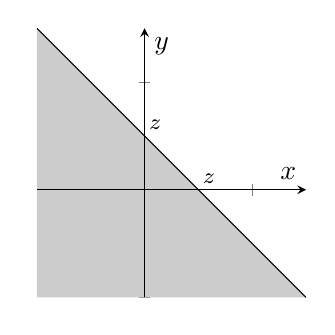
\begin{tikzpicture}
    
            \definecolor{siva}{rgb}{0.8, 0.8, 0.8}
    
            \begin{axis}[
                axis lines = left,
                xlabel = $x$,
                ylabel = $y$,
                domain=-1:2,
                samples=500,
                height=5cm,
                width=5cm,
                xmin=-1, xmax=1.5,
                ymin=-1, ymax=1.5,
                xtick={},
                ytick={},
                xticklabels={},
                yticklabels={},
                axis y line=middle,
                axis x line=middle
            ]
    
            \fill[siva] (-1, 1.5) -- (1.5, -1) -- (-1,-1) -- cycle;

            \draw (-1, 1.5) -- (1.5, -1);
            \draw (-1, 0) -- (1, 0);
            \draw (0, -1) -- (0, 1);
        
            \node at (0.6,0.1) {\footnotesize $z$};
            \node at (0.1,0.6) {\footnotesize $z$};
        
            \end{axis}
        \end{tikzpicture}
    
        \caption{$\{(x,y)  \mid x+y \leq z\}$}
        \label{fig:7}
    \end{figure}
    
    \n Sledi: 
    $$
    f_{X+Y}(z)=\int_{-\infty}^{\infty} f_{(X, Y)}(z-y, y) \, d y
    $$
    Če sta $X$ in $Y$ neodvisni dobimo:
    $$
    f_{X+Y}(z)=\int_{-\infty}^{\infty} f_X(z-y) \cdot f_Y(y) \,d y
    $$
    Slednji pravimo \emph{konvolucija} funkcij $f_X$ in $f_Y$. 
\end{zgled}

\begin{trditev}
    Naj bosta $X$ in $Y$ neodvisni slučajni spremenljivki. $X \sim \chi^2(m)$ in $Y \sim \chi^2(n)$. Potem je: 
    $$
    X+Y \sim \chi^2(m+n)
    $$
\end{trditev}

\begin{proof}
    Vzemimo $X \sim \chi^2(m)$ in $Y \sim \chi^2(n)$. Izračunajmo $X+Y$. Ta je nenegativna (saj je $\chi^2$ negativna) in zato $f_{X+Y}(z)=0$ za $z \leq 0$. Za $z>0$ pa je: 
    \begin{align*}
        f_{X+Y}(z) &= \frac{1}{2^{\frac{m}{2}} \Gamma\left(\frac{m}{2}\right) \cdot 2^{\frac{n}{2}} \Gamma\left(\frac{n}{2}\right)} \int_0^{z} x^{\frac{m}{2}-1} e^{-\frac{x}{2}}(z-x)^{\frac{n}{2}-1} e^{-\frac{z-x}{2}} \, dx \\
        &=\frac{1}{2^{\frac{m+n}{2}} \cdot \Gamma\left(\frac{m}{2}\right) \Gamma\left(\frac{n}{2}\right)} e^{-\frac{z}{2}} \int_0^z x^{\frac{m}{2}-1}(z-x)^{\frac{n}{2}-1} \, d x \tag{$\star$} \\
        &=\frac{1}{2^{\frac{m+n}{2}} \cdot \Gamma\left(\frac{m}{2}\right) \Gamma\left(\frac{n}{2}\right)} e^{-\frac{z}{2}} z^{\frac{m+n}{2}-1} \underbrace{\int_0^1 t^{\frac{m}{2}-1} \cdot(1-t)^{\frac{n}{2}-1} \, d t}_{\beta(\frac{m}{2}, \frac{n}{2}) = \frac{\Gamma\left(\frac{m}{2}\right) \cdot \Gamma\left(\frac{n}{2}\right)}{\Gamma\left(\frac{m}{2}+\frac{n}{2}\right)}} \\
        &=\frac{1}{2^{\frac{m+n}{2}}\Gamma\left(\frac{m+n}{2}\right)} z^{\frac{m+n}{2}-1} e^{-\frac{z}{2}} 
    \end{align*}
    Kjer smo v $(\star)$ vrstici vpeljali novo spremenljivko $tz=x$. Torej je: 
    $$
    X+Y \sim \chi^2(m+n)
    $$
\end{proof}

\begin{posledica}
    Naj bodo neodvisne slučajne spremenljivke $X_1, X_2, \ldots, X_m \sim \operatorname{N}(0,1)$ porazdeljene standardno normalno. Potem je $Y=X_1^2+X_2^2+\ldots+X_n^2 \sim \chi^2(n)$.
\end{posledica}

\begin{proof}
    Vemo že, da je $X_i^2 \sim \chi^2(1)$. Posledica sledi takoj iz trdive, ter trditve da so kvadrati neodvisnih slučajnih spremenljivk med seboj neodvisni.
\end{proof}

\n V splošnem porazdelitev slučajne spremenljivke $h\left(X_1, \ldots, X_n\right)$ najpreprosteje dobimo z dopolnituijo funkcije $h: \mathbb{R}^n \rightarrow \mathbb{R}$ do zvezno diferenciabilne preslikave $g: \mathbb{R}^n \rightarrow \mathbb{R}^n$ (na primer $h(x, y)=x+y$ lahko dopolnimo do $g(x, y)=(x+y, y))$ in izračunamo porazdelitev transformacije $g(X)$.

\begin{trditev}
    Naj bo $X: \Omega \to \mathbb{R}^n$ slučajni vektor z “zvezno” gostoto $f_X:\mathbb{R}^n \to [0, \infty)$. Dalje naj bo $g: \mathbb{R}^n \to \mathbb{R}^n$ (ali $g:D \to E$ za primerni množici $D, E \subseteq \mathbb{R}^n$, kjer $P(X \in D)=1$) zvezno diferenciabilna bijekcija. Tedaj ima slučajni vektor $g(X): \Omega \to \mathbb{R}^n$ gostoto: 
    $$
    f_{g(X)}(z)=f\left(g^{-1}(z)\right) \left\lvert\, \det J_{g^{-1}}(z) \right\rvert =\frac{f\left(g^{-1}(z)\right)}{\left|\det J_g\left(g^{-1}(z)\right)\right|}
    $$
    za vse $z \in \mathbb{R}^n$ (oziroma $z \in E$).
\end{trditev}

\begin{proof}
    Rdeča nit: $P(g(X) \in X)$ želimo izraziti kot $\int_C \ldots$, kjer bo $\ldots$ gostota:
    \begin{align*}
        P(g(X) \in C)&=P\left(X \in g^{-1}(C)\right) \\
        &=\int_{g^{-1}(C)} f_X(x) \, d x \tag{$\star$}\\ 
        &=\int_C f_X\left(g^{-1}(z)\right)\left|\det J_{g^{-1}}(z)\right| \, d z    
    \end{align*} 
    Kjer smo v $(\star)$ vrstici vpeljali novo spremenljivko $x=g^{-1}(z), \, d x=| \det J_{g^{-1}}(z) | d z$.
\end{proof}

\n \textbf{Zapišimo dvorazsežen primer v “tradicionalnih” oznakah:}

\n Transformacijo $g(X, Y)$ zapišemo kot:
$$
(U, V)=(U(X, Y), V(X, Y))
$$
Njen inverz $g^{-1}(U,V)$ pa kot: 
$$
(X, Y)=(X(U, V), Y(U, V))
$$
Tedaj: 
$$
|\det J_{g^{-1}}(u, v)| = \left\lvert\left.\begin{vmatrix}
    \frac{\partial x}{\partial u} & \frac{\partial x}{\partial v} \\
    \frac{\partial y}{\partial u} & \frac{\partial y}{\partial v}
    \end{vmatrix}\right|_{(u, v)} \right\rvert
$$
in
$$
|\det J_{g}(g^{-1}(u, v))| = \left\lvert\left.\begin{vmatrix}
    \frac{\partial u}{\partial x} & \frac{\partial u}{\partial y} \\
    \frac{\partial v}{\partial x} & \frac{\partial v}{\partial y}
    \end{vmatrix}\right|_{(x(u, v), y(u, v))} \right\rvert
$$
Transformacijska formula se tedaj glasi: 
$$
f_{U, V}(u, v)=f_{(X, Y)}(x(u, v), y(u, v)) \cdot \left\lvert\left.\begin{vmatrix}
    \frac{\partial x}{\partial u} & \frac{\partial x}{\partial v} \\
    \frac{\partial y}{\partial u} & \frac{\partial y}{\partial v}
    \end{vmatrix}\right|_{(u, v)} \right\rvert
$$
Upoštevaje $g \circ g^{-1}=\operatorname{id}$ je posledično $J_g\left(g^{-1}(u, v)\right) \cdot J_{g^{-1}}(u, v)=I$. Zgornje lahko prepišemo v: 
$$
f_{U, V}(u, v)=\frac{f_{(X, Y)}(x(u, v), y(u, v))}{\left\lvert\left.\begin{vmatrix}
    \frac{\partial u}{\partial x} & \frac{\partial u}{\partial y} \\
    \frac{\partial v}{\partial x} & \frac{\partial v}{\partial y}
    \end{vmatrix}\right|_{(x(u, v), y(u, v))} \right\rvert}
$$

\begin{zgled}
    ~

    \begin{enumerate}
        \item Oglejmo si transformacijo: 
        $$
        U=X+Y, V=Y \implies Y=V, X=U-V
        $$
        To pomeni $g(x, y)=(x+y, y)$ in $g^{-1}(u, v)=(u-v, v)$. 
        $$
        \det J_g (x,y) = \begin{vmatrix}
            \frac{\partial u}{\partial x} & \frac{\partial u}{\partial y} \\
            \frac{\partial v}{\partial x} & \frac{\partial v}{\partial y}
            \end{vmatrix} = \begin{vmatrix}1 & 1 \\ 0 & 1\end{vmatrix} = 1
        $$
        Torej: 
        $$
        f_{(X+Y, Y)}(u, v)=\frac{f_{(X, Y)}(u-v, v)}{1}
        $$
        Gostota slučajne spremenljivke $X+Y$ je robna gostota oziroma: 
        $$
        f_{X+Y}(u)=\int_{-\infty}^{\infty} f_{(X, Y)}(u-v, v) \, d v
        $$
        \item Oglejmo si še transformacijo: 
        $$
        U=\frac{X}{Y}, V=Y \implies X=U V, Y=V
        $$  
        Pripomnimo, da je transformacija $g(x, y)=\left(\frac{x}{y}, y\right)$ definirana le na $\{Y \neq 0\}=\mathbb{R} \times \mathbb{R} \setminus \{0\}$. Razumemo lahko $g: \mathbb{R} \times \mathbb{R} \setminus\{0\} \to \mathbb{R} \times \mathbb{R} \setminus\{0\}$. Za “zvezen” slučajni vektor $(X,Y)$ seveda velja $P(Y=0)=0$ oziroma $P((X, Y) \in \mathbb{R} \times \mathbb{R} \setminus\{0\})=1$. Po transformacijski formuli velja: 
        $$
        f_{\left(\frac{X}{Y}, Y\right)}(u, v) = \frac{f_{(X, Y)}(u v, v)}{\left\lvert\left.\begin{vmatrix}\frac{1}{y} & * \\ 0 & 1\end{vmatrix}\right|_{y = y(u,v)}\right\rvert} =|v| f_{(X, Y)}(u v, v)
        $$  
        in:
        $$
        f_{\frac{X}{Y}}(u)=\int_{-\infty}^{\infty}|v| f_{(X, Y)}(u v, v) \, d v
        $$
    \end{enumerate}
\end{zgled}

\begin{trditev}
    Naj za $X: \Omega \rightarrow \mathbb{R}^n$ velja $X \sim \operatorname{N}(\mu, \Sigma)$ ($\mu \in \mathbb{R}^n, \Sigma \in \mathbb{R}^{n \times n}$ s.p.d.) in naj bo $A: \mathbb{R}^n \to \mathbb{R}^n$ obrljiva matrika. Dalje naj bo $\nu \in \mathbb{R}^n$. Tedaj: 
    $$
    A X+\nu \sim \operatorname{N}\left(A \mu+\nu, A \Sigma A^{\top}\right)
    $$
\end{trditev}

\begin{proof}
    Imamo $g(x)=A x+\nu$ in $g^{-1}(z)=A^{-1}(z-\nu)$. $g$ je “linearna” (afina) preslikava $\implies J_g(x) \equiv A$. Transformacijska formula pove: 
    \begin{align*}
        f_{A X+\nu}(z)&=\frac{1}{|\det A|} f_X\left(A^{-1}(z-\nu)\right) \\
        &=\frac{1}{\sqrt{|\det A|^2}}(2 \pi)^{-\frac{n}{2}}(\det \Sigma)^{-\frac{1}{2}} e^{-\frac{1}{2}\left\langle\Sigma^{-1}\left(A^{-1}(z - \nu)-\mu\right), A^{-1}(z-\nu)-\mu\right\rangle} \tag{$\star$} \\
        &=(2 \pi)^{-\frac{n}{2}}\left(\det\left(A \Sigma A^{\top}\right)\right)^{-\frac{1}{2}} e^{-\frac{1}{2}\left\langle\left(A^{\top}\right)^{-1} \Sigma^{-1} A^{-1}(z-\nu-A \mu), z-\nu - A\mu\right\rangle} 
    \end{align*}
    V vrstici $(\star)$ velja: 
    $$
    \begin{aligned}
        |\det A|=\sqrt{|\operatorname{det} A|^2}&=\sqrt{\operatorname{del} A \cdot \operatorname{det} A^{\top}}=\sqrt{\operatorname{det}\left(A A^{\top}\right)} \\
         A^{-1}(z-\nu)-\mu&=A^{-1}\left((z-\nu)-A \mu\right)    
    \end{aligned}
    $$
\end{proof}

\begin{posledica}
    Naj bo $X \sim N(\mu, \Sigma)$. Razcepimo $\Sigma=L L^{\top}$ (npr. Cholesky). Sledi, da je $X \sim L Z+\mu$, kjer je $Z \sim N\left(0, I_{n \times n}\right)$ $n$-razsežna standardna normalna porazdelitev. To je klučnega pomena za simulacijo vzorčenja.\footnote[6]{To pomeni, da lahko do katere koli normalne porazdelitve pridemo tako, da naredimo afino preslikavo s spodnje trikotno matriko in nekim vektorjem na standarni normalni porazdelitvi.}
\end{posledica}


\end{document}